\section{Zielsetzung}
Ziel ist es in diesem Versuch, durch Verwendung von Ultraschall, die Geschwindigkeit einer Flüssigkeit, unter verschiedenen Umständen, in einem abgeschlossenen System zu ermitteln.


\section{Theorie}
\label{sec:Theorie}
\subsection{Einleitung}
Ultraschall ist für den Menschen nicht hörbarer Schall im Frequenzbereich zwischen $\SI{20}{\kilo\hertz}$ und ca. $\SI{1}{\giga\hertz}$.
Er entsteht durch Druckschwankungen, wie sie beispielsweise durch einen schwingenden Piezokristall hervorgerufen werden kann.

\subsection{Doppler-Effekt}
Der Doppler-Effekt beschreibt das Phänomen der Frequenzänderung, wenn sich Schallquelle und Empfänger relativ zueinander bewegen.
Im Alltag ist der Doppler-Effekt zu beobachten, wenn z.B. ein Krankenwagen mit eingeschalteter Sirene an einer stehenden Person vorbei fährt.
\subsubsection{Fall 1}
Bewegt sich die Schallquelle auf einen Empfänger mit fester Position zu, vergrößert sich die Grundfrequenz $v_0$ zu $v_\textrm{gr}$.
Sobald sich die Schallquelle entfernt, verkleinert sie sich zu $v_\textrm{kl}$.
Die momentane Frequenz wird durch
\begin{align}
  \nu_\textrm{kl/gr} &= \frac{\nu_0}{1 \pm \frac{\nu}{c}}
  \label{eq:Doppler_1}
\end{align}
bestimmt.
\subsubsection{Fall 2}
Bewegt sich der Empfänger auf eine stehende Quelle zu, vergrößert sich die Frequenz zu $\nu_h$. Entfernt sich der Empfänger von der Quelle, ergibt sich eine tiefere Frequenz $\nu_n$. Dies Verhalten beschreibt die folgende Gleichung.
\begin{align}
  \nu_\textrm{h,n} &= (1 \pm \frac{\nu}{c}) 
  \label{eq:Doppler_2}
\end{align}
\subsection{Dopplereffekt bei Flüssigkeiten}
Der Dopplereffekt wird in diesem Experiment genutzt, um die Geschwindigkeit $v$ einer sich bewegenden Flüssigkeit zu bestimmen. \\
Wie in Abbildung $\ref{fig:Doppler}$ zu sehen, wird die Grundfrequenz $\nu_0$ durch die sich bewegenden Teilchen in der Flüssigkeit nach dem Dopplereffekt verändert. Die Differenz der Frequenzen $\Delta \nu$ wird nach
\begin{align}
  	\Delta \nu = 2\nu_0 \frac{v}{c} \cos{\alpha}
    \label{eq:geschwindigkeit}
\end{align}
berechnet.
Durch die Verwendung des Echo-Impuls-Verfahrens ist die Gleichung nur von dem Einfallswinkel $\alpha$ abhängig.

\begin{figure}
  \centering
  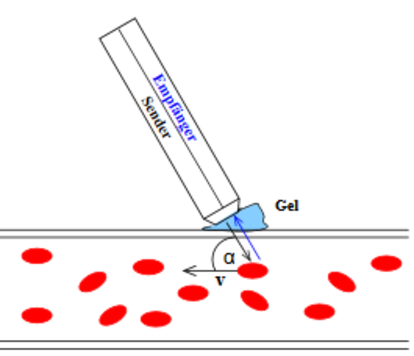
\includegraphics{ressources/Doppler.pdf}
  \caption{Darstellung der Neigung von der Ultraschallsonde zur Flüssigkeit \cite{skript}.}
  \label{fig:Doppler}
\end{figure}



% \begin{figure}[htbp]
%   \begin{minipage}[t]{\textwidth/2}
%       \vspace{0pt}
%       Und nun ein wenig Text $\cdots$ \\
%       Blah, blah, blah, $\cdots$
%     \end{minipage}
%     \begin{minipage}[t]{\textwidth/2}
%       \vspace{0pt}
%       \centering
%       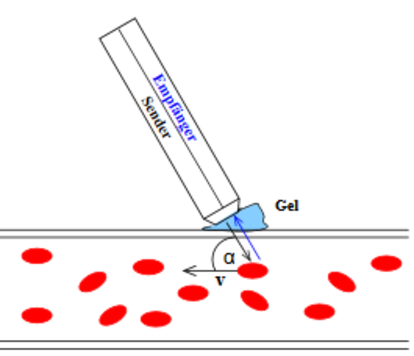
\includegraphics[width=\textwidth]{ressources/Doppler.pdf}
%       \caption{Bild1}
%       \label{fig:Bild1}
%     \end{minipage}
% \hfill
% \end{figure}


% 2x2 Plot
% \begin{figure*}
%     \centering
%     \begin{subfigure}[b]{0.475\textwidth}
%         \centering
%         \includegraphics[width=\textwidth]{Abbildungen/Schaltung1.pdf}
%         \caption[]%
%         {{\small Schaltung 1.}}
%         \label{fig:Schaltung1}
%     \end{subfigure}
%     \hfill
%     \begin{subfigure}[b]{0.475\textwidth}
%         \centering
%         \includegraphics[width=\textwidth]{Abbildungen/Schaltung2.pdf}
%         \caption[]%
%         {{\small Schaltung 2.}}
%         \label{fig:Schaltung2}
%     \end{subfigure}
%     \vskip\baselineskip
%     \begin{subfigure}[b]{0.475\textwidth}
%         \centering
%         \includegraphics[width=\textwidth]{Abbildungen/Schaltung4.pdf}    % Zahlen vertauscht ... -.-
%         \caption[]%
%         {{\small Schaltung 3.}}
%         \label{fig:Schaltung3}
%     \end{subfigure}
%     \quad
%     \begin{subfigure}[b]{0.475\textwidth}
%         \centering
%         \includegraphics[width=\textwidth]{Abbildungen/Schaltung3.pdf}
%         \caption[]%
%         {{\small Schaltung 4.}}
%         \label{fig:Schaltung4}
%     \end{subfigure}
%     \caption[]
%     {Ersatzschaltbilder der verschiedenen Teilaufgaben.}
%     \label{fig:Schaltungen}
% \end{figure*}
